\documentclass[11pt, a4paper]{article}
\usepackage{algpseudocode}

% One of the following is required: problemset, recitation, quiz, exam
% The following are required: handoutnum, assigneddate.
% If there is only one date, set both duedate and assigneddate to be the same.
% Do not change handoutnum or dates
\usepackage[
problemset,
handoutnum=2,
assigneddate={18 September 2021},duedate={28 September 2021},
% % Uncomment the line below IF these are solutions
 solution,
% % Uncomment the line below IF you are a student submitting solutions
student,
% % Replace with your name
name={Neel Bhalla},
% Replace with names of all group members who collarborated on this.
% If unsure about ordering, then you can follow the convention in theory
% and list names alphabetically by last name.
groupmembers={Neel Bhalla, Agnes Shan, Sam Lyon}
]{course-handouts-preamble}

% Be careful of commas and put text with spaces within {curly braces}
% Don't use a comma at the end, but do use commas between options.
% Weird errors occur otherwise, I wasted some time failing to debug those.
% DO NOT EDIT
% These are fixed values that should not be changed during this course.
\pgfkeys{/chp/fixed/.cd,
instructorname = {Ravi Sundaram},
coursename = {CS5800 Algorithms}}

% Add any macros you want below, or put them in a separate file and \input{file}
% keeping the preamble clean can keep you sane.

\begin{document}
% Do not change either of the below lines.
\insertHandoutInfoBox{}
\ifbool{isexam}{\input{exam-blurb}} %comment this line only if it throws an error.

% Start adding content from below here.


\newproblem{Recurrences}{12+8}

\begin{enumerate}[label=\alph*.]

\item \begin{enumerate}
\item
  $T(n) = 3T(n/2) + n$ (This is the recursion for Karatsuba's Algorithm) \\ 
  Observe $\log_2(3) \simeq 1.58 > 1$, thus the majority of the work will occur in the leaves and will have runtime $\Theta(n^{1.58})$

\item
  $T(n) = 3T(n/2) + n^2 $ \\
  Simmilar to above, $\log_2(3) \simeq 1.58 < 2$, thus the majority of the work will be done at the top, and will have runtime $\Theta(n^2)$ \\

\item $T(n) = 2T(n/4) + T(n/2) + n$ (Hint: Think of the number of nodes at each level. You can determine it by solving a recurrence).

We can use recursion tree for this one: \\
  Work done at top level: $n$ with subtasks $\frac{n}{4}$,$\frac{n}{4}$, $\frac{n}{2}$ \\ 
  
  Work done at next level: $n$ with more subtasks. \\ 
 \textbf{Claim}: every level has $n$ work done.  \\ \\
 \textbf{Proof}: Since work done on a level is the amount of data passed in, $n$, it follows that the amount of work done on a level is the amount of data passed in by the recursive subcases.  The amount of data passed down is $2 * \frac{n}{4} + \frac{n}{2} = n$ \\ \\
 Therefore every level will have $n$ work done, and there are $\log n$ levels in the tree, hence $\Theta(n \log n)$ work done.

\item $T(n) = 5T(n/4) + n$ \\ \\
Observe $\log_4(5) = 1.16 > 1$, hence the runtime is $\Theta(n^{1.16})$

\end{enumerate}


\item Use the \textbf{recursion tree method} to solve the following recurrence:

\begin{align*}
T(n) = 3T(n/3) + n; \hspace{0.15in} T(1) = 1
\end{align*}
\begin{figure}
    \centering
    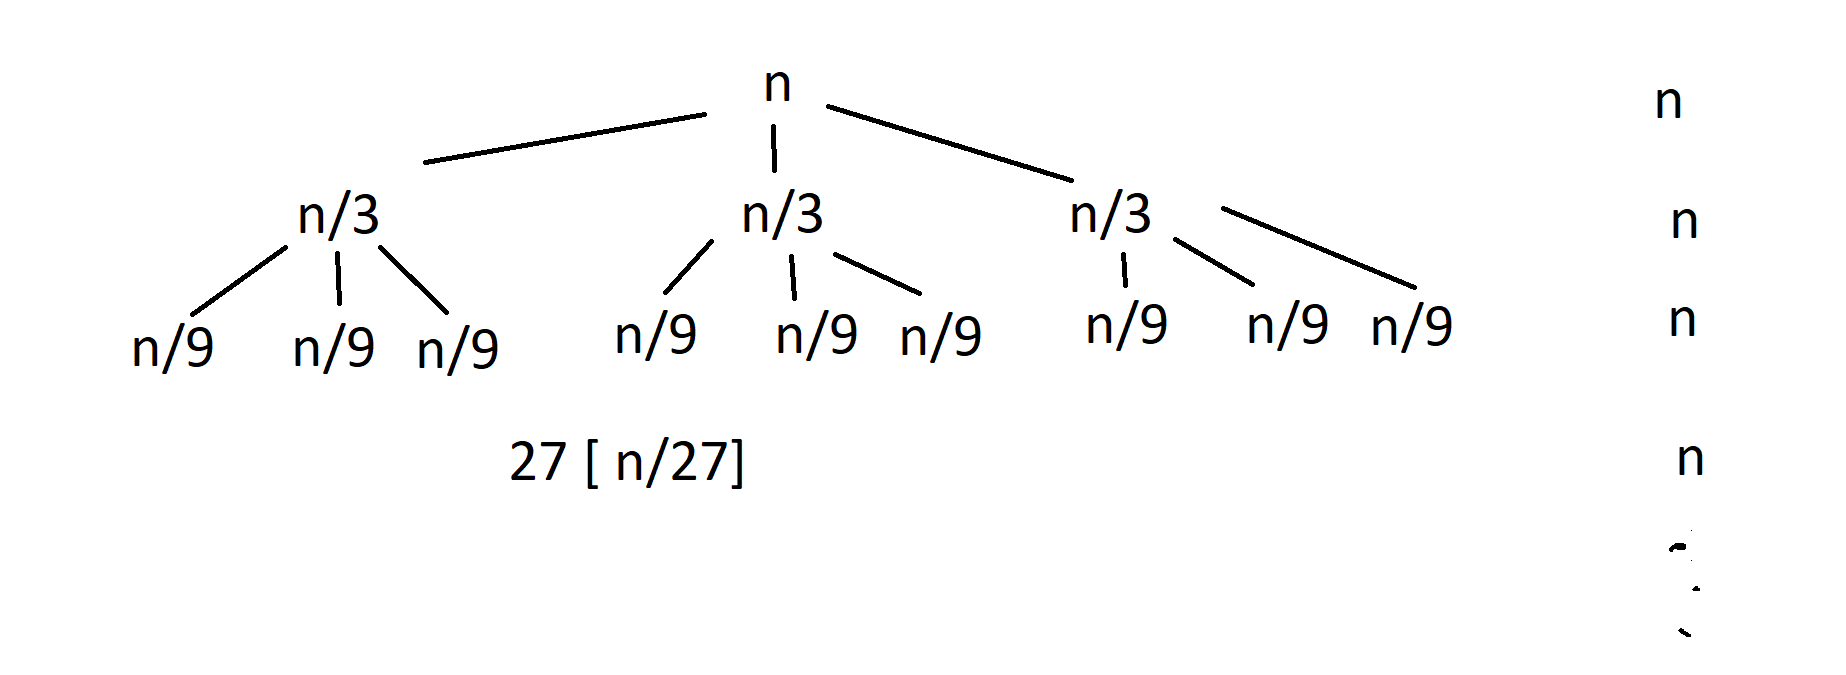
\includegraphics[width=0.5\textwidth]{recursive_trees.png}
    \caption{Recursive work tree, observe every level does $n$ work.}
    \label{fig:my_label}
\end{figure}
Work done at top: $n$ $\to$ three subtasks of $\frac{n}{3}$ \\ 
Work done at next: $3 * \frac{n}{3}$ $\to$ nine subtasks of $\frac{n}{9}$ \\ \\
It is clear that the complexity is
$$\sum_{i = 0}^{\log n} 3^i \frac{n}{3^i}$$
$$= \sum_{i = 0}^{\log n} n = O(n \log n) $$
\end{enumerate}


\newproblem{Rotated and Sorted}{10+10}
Suppose you are given a array of $n$ distinct numbers which was sorted and then rotated $k$ indices, for some unknown integer $k$ between 1 and $n-1$. That is, you are given an array $A[1..n]$ such that some prefix $A[1..k]$ is sorted in increasing order, the corresponding suffix $A[k+1..n]$ is sorted in decreasing order, and $A[n]<A[1]$. For example, you might be given the following 16-element array (where $k=10$): $[9, 13, 16, 20, 21, 24, 25, 26, 27, 30, ||, 1, 2, 3, 5, 6, 8]$
\begin{enumerate}[label=\alph*)]
\item Describe and analyze an algorithm to compute the value of $k$ in $\Theta(\log n)$ time. \\ \\
Since the array is rotated, we know there exists an index $j > 1$ such that $a[j] < a[1]$.  It suffices to find the minimum $j$. \\ \\
Secondly observe that Since the array is rotated, the elements will first be greater than $a[1]$ since they are increasing, and then suddently drop to decreasing and be less than $a[1]$. \\ \\
It suffices to implement a binary search algorithmn to find the minimum $j$ as follows: \\ \\
Since this is binary search on an $n$ element array, it our algorithm must have runtime $\Theta(\log n)$
\begin{algorithm}
\caption{Find the minimum value $j$ such that $a[1] < a[j]$, and return $j-1$ the rotation factor $k$}
\begin{algorithmic}
\Procedure{findRotate}{$arr$}
  \State lo $\leftarrow$ 1
  \State hi $\leftarrow$ $len(arr)$ \Comment{The last element must be less than the first, since it is rotated by at least 1.}
  \While{$lo+1 < hi$}
    \State mid $\leftarrow$ $\floor{\frac{lo+hi}{2}}$
    \If{$a[mid] >= a[1]$}
        \State lo $\leftarrow$ mid
    \Else
      \State hi $\leftarrow$ mid
    \EndIf
  \EndWhile
  \State \Return{$hi-1$} \Comment{If the min index is $j$, the rotation factor is $j-1$}
\EndProcedure
\end{algorithmic}
\end{algorithm}
\item Describe  and  analyze  an  algorithm  to  determine  if  the  given  array contains a given number $x$ that runs in $\Theta(\log n)$ time assuming you already know the value of $k$. \\ \\
If we already know the value of $k$, then we can construct a algorithm to "rotate" an original index to its new place after the rotation.
\begin{algorithm}[h!]
\caption{Compute the new rotated index from index, rotation, and arrlen}
\begin{algorithmic}
\Procedure{rotate}{$ix$,$k$, $arrlen$}
    \State \Return{$(k + ix) \mod arrlen$}
\EndProcedure
\end{algorithmic}
\end{algorithm}
\begin{algorithm}[h!]
\caption{Determine if element is in rotated list}
\begin{algorithmic}
\Procedure{find}{$target$,$k$, $arr$}
\State $arrlen \leftarrow len(arr)$
\If{$arr[rotate(1, k, arrlen)] > target$ or $arr[rotate(arrlen, k, arrlen)] < target$}
    \State \Return{False}
\EndIf
\State $lo \leftarrow 0$ 
\State hi $\leftarrow arrlen+1$
\While{$lo+1 < hi$}
    \State mid $\leftarrow$ $\floor{\frac{lo+hi}{2}}$
    \If{$a[rotate(mid, k, arr)] > target$}
        \State hi $\leftarrow$ mid
    \ElsIf{$a[rotate(mid, k, arr)] = target$}
        \State \Return{True}
    \Else \Comment{less than target}
      \State lo $\leftarrow$ mid
    \EndIf
  \EndWhile
  \State \Return{False}
\EndProcedure
\end{algorithmic}
\end{algorithm}
\\ \\
Utilizing this transformation, it is sufficent to implement standard binary search, but apply the transformation when calculating the "middle element" of the array.(Cont on next page)


\newpage
\textbf{Analysis}: Since this is binary search on an $n$ element array, it our algorithm must have runtime $\Theta(\log n)$
\end{enumerate}

\newproblem{Hex}{20}
Hex is a two-player game played on a diamond-shaped board made up of hexagons.  In the game, one player plays white pieces, while the other plays black, with play alternating between players and placement only allowed on unoccupied hexagons. Alternate sides of the board are designated white and black as shown above, and the goal of the game is to complete a chain of pieces between one player's two sides.

\noindent    Give an algorithm that takes as input the black pieces and white pieces on a board of length $n$ on each side, and determines whether that configuration is a winning configuration for either player. Your algorithm must employ the Union-Find data structure. See accompanying figure for an illustration.

\textbf{Solution}: 
Given a map, we can construct a corresponding disjoint-set-union(dsu) structure where each hexagon corresponds to an object.  \\ \\
We then can define two functions: \\ \\
\textbf{add}: Given a dsu, a new cell, and a color to turn it to, we can update the dsu to reflect the new changes.  This is done by checking the neighbors of the cell, and merging adjacent cells (to the one in question) who have the same color. \\ \\
\begin{algorithm}[h!]
\caption{Adds a claimed cell to the dsu structure}
\begin{algorithmic}
\Procedure{addCell}{$dsu$,$graph$, $cell$, $color$}
\For{\texttt{neighbor of cell in graph}}
    \If{color($neighbor$) is $color$}
    \State $union(dsu, neighbor, cell)$

    \EndIf
\EndFor
\EndProcedure
\end{algorithmic}
\end{algorithm}

\textbf{win}: Given a dsu, we can determine if there exists a winner.  For white, this is done by checking if there exists a cell $c_1 \in $ top, $c_2 \in$ bottom with white and $find(c_1) = find(c_2)$.  For black this is done by checking if there exists a cell $c_1 \in $ left, $c_2 \in$ right with black and $find(c_1) = find(c_2)$ \\ \\
\begin{algorithm}[h!]
\caption{Determines if there is a winner}
\begin{algorithmic}
\Procedure{win}{$dsu$, $graph$}
\For{\texttt{cell c1 in top row of graph}}
    \For{\texttt{cell c2 in bottom row of graph}}
    \If{color(c1) is white and color(c2) is white }
    \If{find(dsu, c1) == find(dsu, c2)}
        \State \Return{white}
    \EndIf
    \EndIf
\EndFor
\EndFor
\For{\texttt{cell c1 in left col of graph}}
    \For{\texttt{cell c2 in right col of graph}}
    \If{color(c1) is black and color(c2) is black }
    \If{find(dsu, c1) == find(dsu, c2)}
        \State \Return{black}
    \EndIf
    \EndIf
\EndFor
\EndFor
\State \Return{neither}
\EndProcedure
\end{algorithmic}
\end{algorithm}
\textbf{winning-config}: Given a graph, we can construct an empty dsu.  Next we will add all cells that are occupied with a color, using our addCell function, and then ask whether there is a winner using \textit{win}.

\begin{algorithm}[h!]
\caption{Determines if there is a winner from a graph}
\begin{algorithmic}
\Procedure{winning-config}{$graph$}
\State $dsu \leftarrow$ empty dsu.
\For{\texttt{cell in graph}}
    \State set parent of cell in dsu to itself.
\EndFor
\For{\texttt{cell in graph}}
    \State addCell(dsu, graph, cell, color(cell))
\EndFor
\State \Return{win(dsu,graph)}
\EndProcedure
\end{algorithmic}
\end{algorithm}
\newpage

\newproblem{Thresholded Inversions and Doctor Manhattan}{20+20}

\begin{enumerate}[label=\alph*.]

\item You'll be given an array of integers $a_i$ and a threshold value $t$ as input, describe and analyze an algorithm to determine the number of threshold inversions in the array. An inversion between indices $i < j$ is a threshold inversion if $a_i > t * a_j$, where $t$ is the threshold value given as input.

\textbf{Solution}: We can utilize an enhanced merge sort procedure to solve this.  \\ \\
Given an array, we can break the array into two subproblems.  At each recursive step, we will: 
\begin{itemize}
    \item If:  trivial (size of 0 or 1), return 0 inversions and return the sorted array.
    \item Else:  Count Inversions and Sort the subarrays via recursive call.
    \item then: Count the number of "cross-inversions" by merging in a specific way (detailed below).  We can return the sum of the cross inversions, and inversions done in the recursive steps alongside the new sorted array.
\end{itemize}
\textbf{Merging sorted lists}: Given two sorted lists $L_1$ and $L_2$, it suffices to merge them as follows. 
\begin{algorithm}[h!]
\caption{Merge two lists}
\begin{algorithmic}
\Procedure{merge}{$l1$, $l2$}
\State answer $\leftarrow$ \{\}
\While{$L_1$ and $L_2$ are not empty}
    \If{$L_1$ is empty}
        \State \Return{answer + $L_2$}
    \ElsIf{$L_2$ is empty}
        \State \Return{answer + $L_1$}
    \Else
        \If{$L_1[1] < L_2[1]$}
            \State append $L_1[1]$ on answer
            \State pop $L_1[1]$ from list.
        \Else
            \State append $L_2[1]$ on answer
            \State pop $L_2[1]$ from list.
        \EndIf
    \EndIf    
\EndWhile
\State \Return{answer}
\EndProcedure
\end{algorithmic}
\end{algorithm}
\\ \\
\textbf{Counting inversions}, Observe that when an element is appended to answer, all elements less than it have already been append.  The only other requirement for an cross-inversion is that it must be from $L_2$, with the first element being from $L_1$ (assuming that all internal inversions within $L_1$ and $L_2$ have been covered in the recursive cases). \\ \\
It follows that we can keep track of the number of elements appended from $L_2$, and add this to the number of cross inversions every time we append an element from $L_1$. \\ \\
\textbf{Including the threshold factor}: Merging and counting inversions are the same when $t=1$, but the order changes for $t > 1$.  This is becuase elements may be less than others, but are not necessarily inversions becuase $t*a[j] > a[i]$, but $a[i] > a[j]$ (for $i < j$) \\ \\
Therefore we will separate the merging step and the inversions step, but "simulate merging" in a thresholded order by merging $L_1$ first iff $L_1[1] < t* L_2[1]$. \\ \\  This guarantees that every element of $L_1$ is eligible to form an inversion for all the already appended elements of $L_2$ at time of appending the original element. \\ \\
\textbf{Cross Inversions Algorithm}:

\begin{algorithm}[h!]
\caption{Count number of cross-t-inversions between two lists.}
\begin{algorithmic}
\Procedure{countInversions}{$l1$, $l2$, $t_{fac}$}
\State l2pass $\leftarrow$ 0
\State inversions $\leftarrow$ 0
\While{$L_1$ and $L_2$ are not empty}
    \If{$L_1$ is empty}
        \State \Return{inversions} \Comment{ cannot create more inversions as no elements in $L_1$}
    \ElsIf{$L_2$ is empty}
        \State \Return{inversions + $len(L_1)*$ l2pass} \State \Comment{All of $L_2$ is commited, so every remaining ele of $L_1$ can make an inversion with  $L_2$}
    \Else
        \If{$L_1[1] <= t_{fac}L_2[1]$}
           
            \State pop $L_1[1]$ from list.
            \State inversions $\leftarrow$  inversions + l2pass
        \Else
            \State pop $L_2[1]$ from list.
            \State l2pass $\leftarrow$ l2pass + 1
        \EndIf`
    \EndIf    
\EndWhile
\State \Return{inversions}
\EndProcedure
\end{algorithmic}
\end{algorithm}
\newpage
\textbf{Analysis}: (Both merge, and count-inv): At every iteration of the loop, one element of either $L_1$ or $L_2$ is removed, hence the loop will only iterate $O(n+m)$ time where $n$ and $m$ are the respective lengths. \\ \\
Therefore at a given level, 
$$T(n) = 2 * T(\frac{n}{2}) + 2n$$
 \\
Observe that $\log_2(2) = 1$, thus there will be equal work done at every level (linear) and it follows that the runtime of this algorithm must be $\Theta(n \log n)$, as requried.
\item \textbf{Description}: Assist Doctor Manhattan in his attempt to preemptively save the world. \\ 
Hackerrank id: \textbf{neelbhallabos}

\end{enumerate}
\end{document}